% IEEE conference paper. Build: latexmk -pdf main.tex   (or upload the paper/ folder to Overleaf)
\documentclass[conference]{IEEEtran}
\IEEEoverridecommandlockouts

\usepackage{cite}
\usepackage{amsmath,amssymb}
\usepackage{graphicx}
\usepackage{booktabs}
\usepackage{tikz}
\usetikzlibrary{positioning,arrows.meta,calc}
\usepackage[hidelinks]{hyperref}

% Numbers produced by the analysis pipeline (src/build_report.py and paper/make_assets.py).
% Generated by src/build_report.py -- do not edit by hand.
\newcommand{\vnMain}{285}
\newcommand{\vnA}{303}
\newcommand{\vnB}{327}
\newcommand{\vrhoMain}{0.283}
\newcommand{\vrhoMainLo}{0.177}
\newcommand{\vrhoMainHi}{0.384}
\newcommand{\vrhoA}{0.260}
\newcommand{\vrhoALo}{0.155}
\newcommand{\vrhoAHi}{0.363}
\newcommand{\vrhoB}{0.305}
\newcommand{\vrhoBLo}{0.205}
\newcommand{\vrhoBHi}{0.399}
\newcommand{\vpAsymMain}{1.2\times10^{-6}}
\newcommand{\vkwH}{26.4}
\newcommand{\vepsSq}{0.093}
\newcommand{\valphaC}{0.89}
\newcommand{\vrTwoBase}{0.004}
\newcommand{\vrTwoProp}{0.086}
\newcommand{\vdRTwo}{0.081}
\newcommand{\vFnested}{24.9}
\newcommand{\vpNested}{< 0.001}
\newcommand{\vbeta}{1.30}
\newcommand{\vbetaLo}{0.81}
\newcommand{\vbetaHi}{1.79}
\newcommand{\vbetaStd}{0.29}
\newcommand{\vbetaStdLo}{0.18}
\newcommand{\vbetaStdHi}{0.40}
\newcommand{\vcatDRTwo}{0.093}
\newcommand{\vshapiroP}{0.001}
\newcommand{\vbpP}{0.18}
\newcommand{\vnLog}{420}
\newcommand{\vnWarm}{60}
\newcommand{\vnBench}{360}
\newcommand{\vnInjected}{25}
\newcommand{\vnPaired}{155}
\newcommand{\vmaxDiff}{2.2e-16}
\newcommand{\vlatBase}{456.4}
\newcommand{\vlatVec}{47.2}
\newcommand{\vspeedTwoEightFive}{9.67}
\newcommand{\vspeedTwoEightFiveLo}{9.27}
\newcommand{\vspeedTwoEightFiveHi}{10.31}
\newcommand{\vspeedMin}{3.3}
\newcommand{\vspeedMax}{27.8}
\newcommand{\vspeedMinN}{2000}
\newcommand{\vspeedMaxN}{50}
\newcommand{\vcpu}{Intel(R) Xeon(R) Processor @ 2.80GHz}
\newcommand{\vncpu}{2}
\newcommand{\vpyBench}{3.12.3}

% Generated by paper/make_assets.py -- do not edit by hand.
\newcommand{\pMedOne}{12.0}
\newcommand{\pMedTwo}{14.0}
\newcommand{\pMedThree}{16.0}
\newcommand{\pMedFour}{15.5}
\newcommand{\pDeltaTwo}{0.21}
\newcommand{\pDeltaTwoCi}{[-0.01, 0.42]}
\newcommand{\pHolmTwo}{0.067}
\newcommand{\pMedDiffTwo}{+2.0}
\newcommand{\pDeltaThree}{0.39}
\newcommand{\pDeltaThreeCi}{[0.23, 0.53]}
\newcommand{\pHolmThree}{<0.001}
\newcommand{\pMedDiffThree}{+4.0}
\newcommand{\pDeltaFour}{0.41}
\newcommand{\pDeltaFourCi}{[0.21, 0.60]}
\newcommand{\pHolmFour}{<0.001}
\newcommand{\pMedDiffFour}{+3.5}
\newcommand{\pDeltaBOne}{0.19}
\newcommand{\pDeltaBOneCi}{[-0.08, 0.45]}
\newcommand{\pHolmBOne}{0.159}
\newcommand{\pMedDiffBOne}{+1.5}
\newcommand{\pDeltaBTwo}{0.36}
\newcommand{\pDeltaBTwoCi}{[0.09, 0.62]}
\newcommand{\pHolmBTwo}{0.032}
\newcommand{\pMedDiffBTwo}{+3.5}
\newcommand{\pDeltaBThree}{0.51}
\newcommand{\pDeltaBThreeCi}{[0.29, 0.69]}
\newcommand{\pHolmBThree}{<0.001}
\newcommand{\pMedDiffBThree}{+4.5}
\newcommand{\pDeltaBFour}{0.54}
\newcommand{\pDeltaBFourCi}{[0.28, 0.76]}
\newcommand{\pHolmBFour}{<0.001}
\newcommand{\pMedDiffBFour}{+5.0}
\newcommand{\pLatLoopFifty}{374.6}
\newcommand{\pLatHighLoopFifty}{430.7}
\newcommand{\pLatVecFifty}{13.5}
\newcommand{\pLatHighVecFifty}{17.9}
\newcommand{\pSpeedFifty}{27.80}
\newcommand{\pSpeedFiftyCi}{[27.02, 28.92]}
\newcommand{\pLatLoopTwoEightyFive}{456.4}
\newcommand{\pLatHighLoopTwoEightyFive}{524.8}
\newcommand{\pLatVecTwoEightyFive}{47.2}
\newcommand{\pLatHighVecTwoEightyFive}{63.7}
\newcommand{\pSpeedTwoEightyFive}{9.67}
\newcommand{\pSpeedTwoEightyFiveCi}{[9.27, 10.31]}
\newcommand{\pLatLoopTwoThousand}{905.3}
\newcommand{\pLatHighLoopTwoThousand}{1065.0}
\newcommand{\pLatVecTwoThousand}{277.3}
\newcommand{\pLatHighVecTwoThousand}{324.7}
\newcommand{\pSpeedTwoThousand}{3.26}
\newcommand{\pSpeedTwoThousandCi}{[3.10, 3.41]}


\begin{document}

\title{Academic Generative AI Use and Unintentional Procrastination: A Reproducible Secondary Analysis with a Benchmarked Bootstrap Pipeline}

\author{\IEEEauthorblockN{Ernur Kussain}
\IEEEauthorblockA{Narxoz University\\
Almaty, Kazakhstan\\
yernur.kussain@narxoz.kz}
\and
\IEEEauthorblockN{Zhanassyl Zhakyp}
\IEEEauthorblockA{Narxoz University\\
Almaty, Kazakhstan\\
zhanassyl.zhakyp@narxoz.kz}}

\maketitle

\begin{abstract}
Generative artificial intelligence (GenAI) has become part of everyday study, yet it is unclear whether frequent academic use goes together with unintentional procrastination. We re-analysed an open survey of Indian bachelor's and master's students with a rank-based analysis plan fixed before estimation. In the main sample ($n=\vnMain$), GenAI-use frequency was positively associated with the Unintentional Procrastination Scale (UPS) total: Spearman $\hat\rho_s=\vrhoMain$ (95\% bootstrap CI \vrhoMainLo--\vrhoMainHi, $p=\vpAsymMain$). The estimate was stable in two independently selected samples ($\hat\rho_s=\vrhoA$ and \vrhoB). Students using GenAI a few times a week or daily scored 3.5--4 points higher than the lowest-use reference group (Cliff's $\delta\approx0.4$), and frequency raised explained variance over a demographic baseline model from $R^2=\vrTwoBase$ to \vrTwoProp. All results come from a tested pipeline with data-quality guardrails; replacing its loop bootstrap with a vectorised one cut median latency \vspeedTwoEightFive-fold at the study's sample size while returning identical estimates. Within this cross-sectional design the association is modest and cannot be read causally. We discuss what the Indian estimate implies, and does not imply, for students in Kazakhstan.
\end{abstract}

\begin{IEEEkeywords}
generative artificial intelligence, unintentional procrastination, higher education, Spearman correlation, bootstrap, reproducible research
\end{IEEEkeywords}

\section{Introduction}

Large language models moved into higher education within a few semesters, and students now use them to draft, summarise and debug their coursework~\cite{kasneci2023chatgpt}. Their effect on study behaviour is less clear. Procrastination, the voluntary delay of an intended action despite expected costs, is a well-documented self-regulatory failure among students~\cite{steel2007nature}. Its unintentional form, captured by the Unintentional Procrastination Scale (UPS), describes losing track of tasks rather than deliberately postponing them~\cite{fernie2017ups}. Because a GenAI tool can complete a task within minutes, frequent use could plausibly make late starts feel less costly.

Evidence on this link is mixed. In a cross-sectional study of university students, GenAI usage was associated with higher procrastination ($\beta=0.309$)~\cite{abbas2024harmful}, whereas a three-wave panel that controlled for baseline procrastination found that use frequency did not predict later procrastination ($\beta=0.007$)~\cite{zhao2026panel}. Studies from Kazakhstan document wide adoption: 65\% of 840 surveyed students used AI tools for study at least weekly~\cite{askarkyzy2024perceptions}, and continuance intention has been modelled for academic writing~\cite{bekturova2025tefl}. We found no study that relates the frequency of use to procrastination there.

Three gaps follow. First, reported associations rarely state what they are compared with: a null value, a lowest-use group or a demographic model. Second, the analysis code behind such estimates is seldom published or tested, so it is hard to tell whether a result depends on preprocessing choices. Third, Kazakhstani evidence is absent, so local discussion relies on estimates from other countries.

We address these gaps with a secondary analysis of an open survey of Indian students~\cite{sharma2026dataset}, analysed with rank-based statistics and a pipeline that stops when data-quality checks fail. We ask three research questions:
\begin{itemize}
\item \textbf{RQ1:} Is academic GenAI-use frequency monotonically associated with the UPS total?
\item \textbf{RQ2:} How large is the association relative to a lowest-use reference group and to a demographic baseline model?
\item \textbf{RQ3:} Can the bootstrap pipeline be vectorised without changing its estimates, and with what latency gain?
\end{itemize}

Our contributions are:
\begin{itemize}
\item an estimate of the association with bootstrap and permutation inference, re-estimated in two independently selected samples;
\item a comparison against five explicit baselines, including a lowest-use reference group and a demographic model;
\item an open, tested pipeline with guardrails and a benchmark showing that vectorisation preserves estimates to machine precision;
\item a discussion of how far the Indian estimate can be transferred to Kazakhstan.
\end{itemize}

Section~\ref{sec:method} describes the data, estimators and pipeline. Section~\ref{sec:results} reports the results and discusses them in Section~\ref{sec:discussion}, and Section~\ref{sec:conclusion} states the limitations and concludes.

\section{Methodology}\label{sec:method}

Fig.~\ref{fig:arch} gives an overview of the pipeline, and Table~\ref{tab:params} lists its fixed parameters.

\subsection{Data and Samples}\label{sec:data}
The source is version~1 of an open Mendeley Data record of Indian undergraduate and postgraduate students~\cite{sharma2026dataset}, licensed CC~BY~4.0. It contains a raw workbook with 355 responses and a cleaned workbook with 300. Both files are verified against their published SHA-256 hashes before use. For respondent $i$, the exposure $x_i\in\{1,2,3,4\}$ is the reported frequency of academic GenAI use (a few times a month, once a week, a few times a week, every day), and the target is the UPS total
\begin{equation}
y_i=\sum_{k=1}^{6}u_{ik}\in\{6,\dots,24\},\qquad u_{ik}\in\{1,2,3,4\}, \label{eq:ups}
\end{equation}
where $u_{ik}$ is the coded answer to item $k$. Recomputed totals matched the totals supplied by the data authors in all 300 cleaned records, and the items were internally consistent (Cronbach's $\alpha=\valphaC$~\cite{cronbach1951alpha}).

The main sample keeps the \vnMain{} cleaned records of bachelor's and master's students and excludes 15 higher-secondary respondents. Because the authors' reasons for removing 55 raw records are not documented, Sensitivity~A re-selects eligible raw records with our own rules ($n=\vnA$). Sensitivity~B additionally keeps the 24 respondents who use GenAI rarely or never as level~0 ($n=\vnB$), which provides a lowest-use group that the main sample lacks.

\subsection{Estimators and Baselines}\label{sec:estimators}
The primary metric is Spearman's rank correlation~\cite{spearman1904proof},
\begin{equation}
\hat\rho_s=\operatorname{corr}\bigl(R(\mathbf{x}),R(\mathbf{y})\bigr), \label{eq:rho}
\end{equation}
the Pearson correlation of mid-ranks $R(\cdot)$, which suits an ordinal exposure and a non-normal target. We test $H_0\colon\rho_s=0$ against $H_1\colon\rho_s\neq0$ at $\alpha=0.05$ (two-sided). Uncertainty is quantified with a paired percentile bootstrap~\cite{efron1979bootstrap}: respondents are resampled with replacement $B$ times, and
\begin{equation}
\mathrm{CI}_{95\%}=\bigl[Q_{0.025}(\{\hat\rho^{*}_{b}\}),\;Q_{0.975}(\{\hat\rho^{*}_{b}\})\bigr], \label{eq:ci}
\end{equation}
where resamples with a constant variable are skipped and at least 95\% must remain valid. A permutation test shuffles $\mathbf{y}$ $B$ times:
\begin{equation}
p_{\text{perm}}=\frac{1+\#\bigl\{b\colon|\hat\rho_s(\mathbf{x},\mathbf{y}_{\pi_b})|\ge|\hat\rho_s(\mathbf{x},\mathbf{y})|\bigr\}}{B+1}. \label{eq:perm}
\end{equation}

Five baselines frame the estimate: (i)~the null value $\rho_s=0$; (ii)~a lowest-use reference group (a few times a month in the main sample, rarely or never in Sensitivity~B), compared with each higher level by the Mann--Whitney test, Cliff's $\delta$~\cite{cliff1993dominance} and Holm correction~\cite{holm1979simple}, after an omnibus Kruskal--Wallis test~\cite{kruskal1952ranks}; (iii)~a demographic model; (iv)~the published estimate of Abbas et al.~\cite{abbas2024harmful}; and (v)~for the pipeline, the original loop implementation. Baseline~(iii) is the model $M_0$ in
\begin{equation}
M_0\colon y_i=\mathbf{z}_i^{\top}\boldsymbol\gamma+\varepsilon_i,\qquad M_1\colon y_i=\mathbf{z}_i^{\top}\boldsymbol\gamma+\beta x_i+\varepsilon_i, \label{eq:models}
\end{equation}
where $\mathbf{z}_i$ holds age, gender and education. Both are fitted by ordinary least squares, i.e.\ by minimising $\mathcal{L}=\frac{1}{n}\sum_i(y_i-\hat y_i)^2$, with HC3 standard errors~\cite{long2000hc}; the nested $F$-test and $\Delta R^2$ measure what $x_i$ adds. Table~\ref{tab:baselines} and Fig.~\ref{fig:effects} report the estimates against these baselines.

\subsection{Pipeline, Guardrails and Benchmark}\label{sec:pipeline}
In Fig.~\ref{fig:arch}, one command runs every stage from a single configuration file, and metric points M1--M6 record hashes, exclusions, timings, estimates and output checks. The analysis stops if any guardrail fails: invalid or missing item values, duplicate identifiers, totals outside 6--24, a mismatch with the supplied totals, a constant variable, or fewer than 95\% valid bootstrap resamples.

\begin{figure}[!t]
\centering
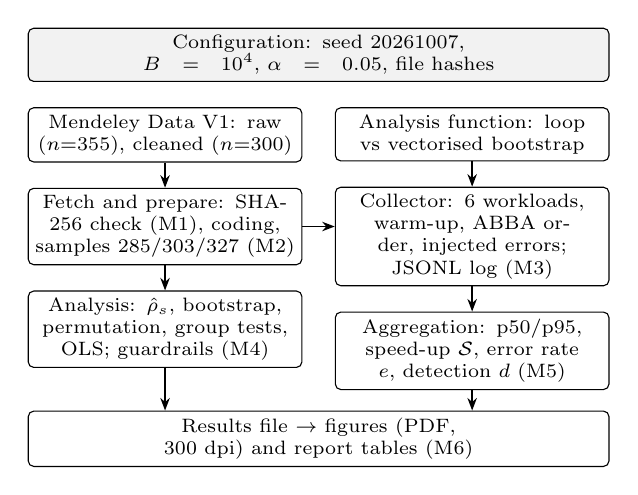
\begin{tikzpicture}[
  box/.style={draw, rounded corners=2pt, align=center, font=\scriptsize, inner sep=2.5pt, minimum height=6.5mm, text width=33mm},
  arr/.style={-{Stealth[length=1.6mm]}, semithick},
  node distance=3.2mm and 4mm]
\node[box, text width=72mm, fill=black!5] (cfg) {Configuration: seed 20261007, $B=10^4$, $\alpha=0.05$, file hashes};
\node[box, below=of cfg.south west, anchor=north west] (src) {Mendeley Data V1: raw ($n{=}355$), cleaned ($n{=}300$)};
\node[box, below=of src] (prep) {Fetch and prepare: SHA-256 check (M1), coding, samples 285/303/327 (M2)};
\node[box, below=of prep] (ana) {Analysis: $\hat\rho_s$, bootstrap, permutation, group tests, OLS; guardrails (M4)};
\node[box, below=of cfg.south east, anchor=north east] (impl) {Analysis function: loop vs vectorised bootstrap};
\node[box, below=of impl] (col) {Collector: 6 workloads, warm-up, ABBA order, injected errors; JSONL log (M3)};
\node[box, below=of col] (agg) {Aggregation: p50/p95, speed-up $\mathcal{S}$, error rate $e$, detection $d$ (M5)};
\node[box, text width=72mm, below=4mm of $(ana.south)!0.5!(agg.south)$] (out) {Results file $\rightarrow$ figures (PDF, 300 dpi) and report tables (M6)};
\draw[arr] (src) -- (prep);
\draw[arr] (prep) -- (ana);
\draw[arr] (impl) -- (col);
\draw[arr] (col) -- (agg);
\draw[arr] (ana.south) -- (ana.south |- out.north);
\draw[arr] (agg.south) -- (agg.south |- out.north);
\draw[arr] (prep.east) -- (impl.west |- prep.east);
\end{tikzpicture}
\caption{Pipeline architecture. Left: survey analysis; right: performance benchmark of the same analysis function. M1--M6 mark where metrics are recorded; the analysis stops when a guardrail fails.}
\label{fig:arch}
\end{figure}

The benchmark times one complete analysis call (validation, scoring and a $10^3$-resample bootstrap) for two implementations: the original loop, which calls the rank correlation once per resample, and a vectorised version that ranks blocks of up to 2{,}000 resamples at once with NumPy~\cite{harris2020numpy} while drawing identical resample indices. Workloads of 50--2{,}000 records are resampled from the real data. Each condition has 5 discarded warm-up runs and 30 timed runs in alternating ABBA order, and each timed repetition receives an invalid batch with probability 0.1. With $\tilde L$ denoting median latency, the primary engineering metric is
\begin{equation}
\mathcal{S}(w)=\tilde L_{\text{loop}}(w)\,/\,\tilde L_{\text{vec}}(w), \label{eq:speedup}
\end{equation}
complemented by the unexpected-error rate $e$, the rejection rate $d$ of injected batches and the largest absolute difference between the two implementations' estimates.

\begin{table}[!t]
\caption{Fixed Analysis and Benchmark Parameters}
\label{tab:params}
\centering
\footnotesize
\begin{tabular}{@{}ll@{}}
\toprule
Parameter & Value \\
\midrule
Seed; significance level & 20261007; $\alpha=0.05$, two-sided \\
Bootstrap / permutation resamples & $B=10{,}000$ each \\
Minimum valid bootstrap fraction & 0.95 \\
Benchmark bootstrap resamples & 1{,}000 per analysis call \\
Workloads (records per run) & 50, 100, 285, 500, 1{,}000, 2{,}000 \\
Runs per condition & 5 warm-up (discarded) + 30 timed \\
Injected invalid batches & probability 0.1 per repetition, 4 types \\
Agreement tolerance & $|\Delta\hat\rho_s|\le10^{-9}$ \\
\bottomrule
\end{tabular}
\end{table}

\section{Results and Discussion}\label{sec:results}

\subsection{Experimental Setup}
The analysis ran in Python with NumPy~2.3.5, SciPy~1.17.0, pandas~2.3.3 and statsmodels~0.14.5 from a pinned lock file. Thirty unit tests pass, and a Docker build and a fresh-clone run reproduced the committed estimates. The benchmark log holds \vnLog{} records (\vnWarm{} warm-up, \vnBench{} timed) collected on an \vcpu{} with \vncpu{} logical CPUs and Python~\vpyBench.

\subsection{RQ1: Association}
In the main sample, GenAI-use frequency and the UPS total~\eqref{eq:ups} were positively associated: $\hat\rho_s=\vrhoMain$ by~\eqref{eq:rho}, 95\% CI \vrhoMainLo--\vrhoMainHi{} by~\eqref{eq:ci}, asymptotic $p=\vpAsymMain$. No permutation in~\eqref{eq:perm} reached the observed value, so $p_{\text{perm}}=1/(B+1)\approx10^{-4}$, and all $10^4$ bootstrap resamples were valid. $H_0$ is therefore rejected. Fig.~\ref{fig:effects} shows that the estimate barely moved in Sensitivity~A ($\hat\rho_s=\vrhoA$) and Sensitivity~B ($\hat\rho_s=\vrhoB$), the two alternative selections of Section~\ref{sec:data}, so the result does not appear to depend on the data authors' undocumented exclusions.

\begin{figure}[!t]
\centering
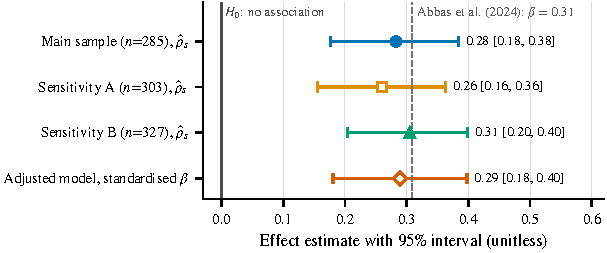
\includegraphics[width=\columnwidth]{generated/fig_effects.pdf}
\caption{Effect estimates with 95\% intervals: Spearman $\hat\rho_s$ in the three samples (bootstrap) and the standardised $\beta$ of model $M_1$ (HC3). The solid line is the null baseline; the dashed line is the estimate of Abbas et al.~\cite{abbas2024harmful}.}
\label{fig:effects}
\end{figure}

\subsection{RQ2: Comparison with Baselines}
Table~\ref{tab:baselines} compares the estimate with the statistical baselines of Section~\ref{sec:estimators}. The four frequency groups differed overall (Kruskal--Wallis $H=\vkwH$, $p<0.001$, $\varepsilon^2=\vepsSq$). Relative to the monthly reference group (median \pMedOne), students using GenAI a few times a week or every day scored 3.5--4 points higher with medium dominance ($\delta=\pDeltaThree$ and \pDeltaFour), while weekly users did not differ after Holm correction. Against the rarely-or-never group of Sensitivity~B, the corresponding $\delta$ rose to \pDeltaBThree{} and \pDeltaBFour. Adding frequency to the demographic model~\eqref{eq:models} raised $R^2$ from \vrTwoBase{} to \vrTwoProp{} ($F=\vFnested$, $p\vpNested$); each step up the frequency scale corresponded to $\beta=\vbeta$ UPS points (95\% CI \vbetaLo--\vbetaHi). The residuals were not normal (Shapiro--Wilk $p=\vshapiroP$), which supports the rank-based primary metric and the HC3 errors, and showed no clear heteroscedasticity (Breusch--Pagan $p=\vbpP$).

\begin{table}[!t]
\caption{Survey Estimates Against the Statistical Baselines}
\label{tab:baselines}
\centering
\footnotesize
\setlength{\tabcolsep}{3pt}
\begin{tabular}{@{}llll@{}}
\toprule
Baseline & Proposed & Estimate [95\% CI] & $p$ \\
\midrule
$\rho_s=0$ & Main, $\hat\rho_s$ & \vrhoMain{} [\vrhoMainLo, \vrhoMainHi] & $\vpAsymMain$ \\
$\rho_s=0$ & Sens.\ A, $\hat\rho_s$ & \vrhoA{} [\vrhoALo, \vrhoAHi] & $<0.001$ \\
$\rho_s=0$ & Sens.\ B, $\hat\rho_s$ & \vrhoB{} [\vrhoBLo, \vrhoBHi] & $<0.001$ \\
Monthly & Weekly, $\delta$ & $\pDeltaTwo$ $\pDeltaTwoCi$ & $\pHolmTwo^{\dagger}$ \\
(median \pMedOne) & Few/week, $\delta$ & $\pDeltaThree$ $\pDeltaThreeCi$ & $\pHolmThree^{\dagger}$ \\
 & Daily, $\delta$ & $\pDeltaFour$ $\pDeltaFourCi$ & $\pHolmFour^{\dagger}$ \\
$M_0$, $R^2=\vrTwoBase$ & $M_1$, $\Delta R^2$ & \vdRTwo{} ($R^2=\vrTwoProp$) & $<0.001$ \\
Abbas et al., $\beta=0.31$ & Std.\ $\beta$ & \vbetaStd{} [\vbetaStdLo, \vbetaStdHi] & --- \\
\bottomrule
\multicolumn{4}{@{}l@{}}{\scriptsize $^{\dagger}$Holm-adjusted Mann--Whitney $p$; $\delta$ is Cliff's dominance.}\\
\end{tabular}
\end{table}

\subsection{RQ3: Pipeline Performance}
Table~\ref{tab:bench} and Fig.~\ref{fig:latency} compare the two implementations under the design of Section~\ref{sec:pipeline}. The vectorised bootstrap was faster at every workload, with $\mathcal{S}$ in~\eqref{eq:speedup} falling from \vspeedMax{} at 50 records to \vspeedMin{} at 2{,}000. The loop pays a fixed cost of one library call per resample, which dominates small inputs; as $n$ grows, ranking itself dominates both versions and the gap narrows. Over \vnPaired{} paired runs on identical inputs, the largest difference between the estimates was $2.2\times10^{-16}$, no run failed unexpectedly ($e=0$), and all \vnInjected{} injected invalid batches were rejected ($d=1$).

\begin{table}[!t]
\caption{Median (p95) Latency per Analysis Call in ms}
\label{tab:bench}
\centering
\footnotesize
\begin{tabular}{@{}rccc@{}}
\toprule
Records & Loop (baseline) & Vectorised & Speed-up $\mathcal{S}$ [95\% CI] \\
\midrule
50 & \pLatLoopFifty{} (\pLatHighLoopFifty) & \textbf{\pLatVecFifty} (\pLatHighVecFifty) & \pSpeedFifty{} \pSpeedFiftyCi \\
285 & \pLatLoopTwoEightyFive{} (\pLatHighLoopTwoEightyFive) & \textbf{\pLatVecTwoEightyFive} (\pLatHighVecTwoEightyFive) & \pSpeedTwoEightyFive{} \pSpeedTwoEightyFiveCi \\
2{,}000 & \pLatLoopTwoThousand{} (\pLatHighLoopTwoThousand) & \textbf{\pLatVecTwoThousand} (\pLatHighVecTwoThousand) & \pSpeedTwoThousand{} \pSpeedTwoThousandCi \\
\bottomrule
\end{tabular}
\end{table}

\begin{figure}[!t]
\centering
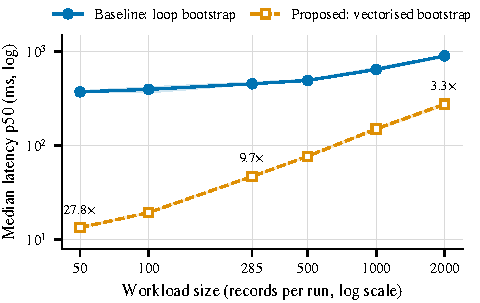
\includegraphics[width=\columnwidth]{generated/fig_latency.pdf}
\caption{Median latency against workload size (log--log). Shaded bands are 95\% bootstrap intervals of the median; labels give the speed-up $\mathcal{S}$.}
\label{fig:latency}
\end{figure}

\subsection{Discussion}\label{sec:discussion}
The results suggest a positive but modest association. By norms for individual-differences research, $\hat\rho_s\approx0.28$ sits near the ``relatively large'' range~\cite{gignac2016effect}, yet frequency explained only about 8\% of the variance in UPS totals. The estimate agrees with the cross-sectional $\beta=0.309$ of Abbas et al.~\cite{abbas2024harmful}, which lies inside our interval (Fig.~\ref{fig:effects}). The panel evidence~\cite{zhao2026panel}, however, implies that a correlation of this size may reflect stable individual differences, such as workload or self-regulation, rather than an effect of GenAI on procrastination. The plateau between use a few times a week and daily use points in the same direction: more frequent use was not associated with ever higher scores.

For Kazakhstan, the estimate is best treated as a hypothesis. With most students already using AI weekly~\cite{askarkyzy2024perceptions}, exposure would be concentrated in the upper levels, a range restriction that would tend to attenuate $\rho_s$. Within our experimental envelope, the engineering result is clearer: removing per-resample library calls gives a three- to 28-fold latency gain without changing a single reported estimate.

These findings have a practical reading. Usage frequency alone appears to be a weak marker of procrastination risk, so policies that simply restrict how often students may use GenAI are unlikely to address the behaviour. Guidance on the purpose of use and support for self-regulation, which the panel evidence links to later academic functioning~\cite{zhao2026panel}, seem more promising targets. For researchers, the pipeline shows that a full bootstrap analysis of a few hundred respondents can run in under a second, which makes repeated sensitivity analyses cheap enough to report routinely.

\section{Limitations and Conclusion}\label{sec:conclusion}

\subsection{Threats to Validity}\label{sec:threats}
\emph{Internal validity.} The survey is cross-sectional and self-reported, so temporal order cannot be established, reverse causation (procrastinators turning to GenAI near deadlines) is plausible, and both measures share one questionnaire, which may inflate their correlation~\cite{podsakoff2003common}. Only age, gender and education were available as covariates; workload, stress and self-regulation remain unmeasured confounders. \emph{Statistical conclusion validity.} With $n=285$, the test had about 80\% power to detect $\rho_s\approx0.17$, and the three group contrasts were Holm-corrected; the sensitivity samples are not independent replications, because they share most respondents. \emph{Construct validity.} Exposure is a single frequency item that ignores the purpose of use, and the UPS measures unintentional rather than academic procrastination~\cite{fernie2017ups}. \emph{External validity.} The data are a convenience sample of Indian students collected for a study of academic dishonesty~\cite{sharma2026dataset}; the estimate does not transfer directly to Kazakhstan. The latency figures come from one two-core machine and from 1{,}000 rather than 10{,}000 resamples per call; absolute times will differ elsewhere, although the guardrail and agreement results should not depend on hardware.

\subsection{Conclusion and Future Work}
Subject to the threats in Section~\ref{sec:threats}, the answers are as follows. For RQ1, academic GenAI-use frequency was positively and robustly associated with unintentional procrastination ($\hat\rho_s=\vrhoMain$), and the estimate was stable under two alternative sample selections (\vrhoA{} and \vrhoB). For RQ2, the association is modest: frequent users scored 3.5--4 points higher than the lowest-use group, and frequency added about 8\% of explained variance to a demographic model. For RQ3, vectorising the bootstrap reduced median latency by a factor of \vspeedMin--\vspeedMax{} while reproducing every estimate.

Future work should (i)~validate Kazakh and Russian versions of the UPS, (ii)~follow students in Kazakhstan over three waves to separate the temporal order of use and procrastination, and (iii)~measure the purpose of GenAI use and behavioural deadline data alongside frequency. The code, data derivatives and validation record are available at \url{https://github.com/yernurkussain-source/TASK2_KUSSAIN_ZHAHYP}.


\bibliographystyle{IEEEtran}
\bibliography{references}

\end{document}
